\chapter{Εισαγωγή}

%Το \en{Lorem Ipsum} είναι απλά ένα κείμενο χωρίς νόημα για τους επαγγελματίες της τυπογραφίας και στοιχειοθεσίας \cite{LoremIpsumAll}. Το \en{Lorem Ipsum} είναι το επαγγελματικό πρότυπο όσον αφορά το κείμενο χωρίς νόημα, από τον 15ο αιώνα, όταν ένας ανώνυμος τυπογράφος πήρε ένα δοκίμιο και ανακάτεψε τις λέξεις για να δημιουργήσει ένα δείγμα βιβλίου. Όχι μόνο επιβίωσε πέντε αιώνες, αλλά κυριάρχησε στην ηλεκτρονική στοιχειοθεσία, παραμένοντας με κάθε τρόπο αναλλοίωτο. Έγινε δημοφιλές τη δεκαετία του '60 με την έκδοση των δειγμάτων της \en{Letraset} όπου περιελάμβαναν αποσπάσματα του \en{Lorem Ipsum}, και πιο πρόσφατα με το λογισμικό ηλεκτρονικής σελιδοποίησης όπως το \en{Aldus PageMaker} που περιείχαν εκδοχές του \en{Lorem Ipsum}.
Ο χρόνος που απαιτείται για τις χειροκίνητες ρυθμίσεις σε δικτυακές συσκευές, όπως η διαμόρφωση των ρυθμίσεων ή η 
ενημέρωση λιστών πρόσβασης, είναι ιδιαίτερα σημαντικός. Η εποχή της χειροκίνητης διαχείρισης φαίνεται να πλησιάζει στο τέλος της, καθώς όλο και 
περισσότερες επιχειρήσεις αναγνωρίζουν τα οφέλη της αυτοματοποίησης. Με κάθε ώρα επένδυσης στον αυτοματισμό εξοικονομούνται πολλές ώρες εργασίας, 
απελευθερώνοντας τους μηχανικούς δικτύου από επαναλαμβανόμενες διαδικασίες.

Ο αυτοματισμός επιτρέπει τον προγραμματισμό και τη διαμόρφωση εκατοντάδων συσκευών σε ελάχιστο χρόνο, μειώνοντας την πιθανότητα 
σφαλμάτων που προκύπτουν από ανθρώπινο λάθος και ενισχύοντας τη δυνατότητα καταγραφής αλλαγών διαμόρφωσης. Ακόμη, δίνει τη δυνατότητα σε ομάδες χωρίς 
εξειδικευμένες γνώσεις δικτύωσης να διαμορφώνουν και να προσαρμόζουν συσκευές σύμφωνα με τις ανάγκες του οργανισμού. Για παράδειγμα, μια επιχείρηση μπορεί 
να εκχωρήσει αυτές τις εργασίες σε ομάδες λειτουργίας χωρίς εξειδικευμένη γνώση δικτύωσης, χρησιμοποιώντας απλώς μια απλή εισαγωγή δεδομένων σε μια εφαρμογή 
ιστού. Ο κώδικας της αυτοματοποίησης αναλαμβάνει όλες τις τεχνικές λεπτομέρειες, εξασφαλίζοντας αξιοπιστία και ταχύτητα στην υλοποίηση των διαμορφώσεων.

Η αυτοματοποίηση έχει επίσης τεράστιο αντίκτυπο στη συντήρηση και στην παρακολούθηση δικτυακών υποδομών, επιτρέποντας στους μηχανικούς να 
λαμβάνουν αναφορές σε πραγματικό χρόνο για την υγεία του δικτύου και την κατάσταση των συσκευών και των πόρτων. Οι καθημερινές και επαναλαμβανόμενες 
εργασίες που απαιτούν τη συλλογή δεδομένων είναι ιδανικές για αυτοματοποίηση, καθώς η αυτόματη αναζήτηση και επεξεργασία των απαιτούμενων πληροφοριών 
δίνει τη δυνατότητα στους μηχανικούς να εξοικονομούν πολύτιμο χρόνο και να μειώνουν την ανάγκη για χειροκίνητη πρόσβαση σε πολλαπλές συσκευές.

Οι πρακτικές αυτοματοποίησης δικτύων υπάρχουν εδώ και χρόνια στον τομέα της διαχείρισης βλαβών και της παρακολούθησης επιπέδου υπηρεσιών, ωστόσο 
οι αυξανόμενες ανάγκες των σύγχρονων επιχειρήσεων καθιστούν αναγκαία τη διαρκή ανάπτυξη νέων λύσεων και ευκαιριών αυτοματισμού. Η ταχεία ανάπτυξη των 
επιχειρηματικών δικτύων και η εισαγωγή νέων τεχνολογιών, όπως το Διαδίκτυο των Πραγμάτων (\en{IoT}) και το υπολογιστικό νέφος, απαιτούν πλέον ισχυρότερη και 
πιο ευέλικτη δικτυακή υποδομή, γεγονός που αυξάνει το φόρτο εργασίας για τους διαχειριστές δικτύων.

Οι παραδοσιακές μέθοδοι, πέρα από χρονοβόρες, απαιτούσαν εξειδικευμένες γνώσεις σε συγκεκριμένα πρωτόκολλα και τεχνολογίες. Για να μειώσουν τα 
λειτουργικά κόστη και να αυξήσουν την αποδοτικότητα, οι μηχανικοί δικτύου εισήγαγαν τον αυτοματισμό δικτύων, υποστηριζόμενοι από μια κοινότητα 
ανοιχτού κώδικα και κορυφαίες εταιρείες, όπως η \en{Cisco}. Χάρη σε εργαλεία όπως η γλώσσα προγραμματισμού \en{Python} και πρωτόκολλα επικοινωνίας, όπως το 
\en{SSH} και το \en{REST}, έχουν αναπτυχθεί εφαρμογές που διευκολύνουν τη σύνδεση και τη διαχείριση πολλαπλών δικτυακών συσκευών.

Επιπλέον, η εισαγωγή της λογικής των \en{microservices} στον τομέα της πληροφορικής έχει δημιουργήσει νέες δυνατότητες, επιτρέποντας τον 
σχεδιασμό αξιόπιστων, ευέλικτων και ευπροσάρμοστων λύσεων αυτοματοποίησης. Μέσω της χρήσης τεχνολογιών διαχείρισης \en{microservices}, όπως το \en{Kubernetes} 
και τα \en{containers}, διασφαλίζεται η μεγαλύτερη ευελιξία και ανεξαρτησία των υπηρεσιών, προσφέροντας τη δυνατότητα στις επιχειρήσεις να προσαρμόζουν τα 
συστήματά τους σύμφωνα με τις μεταβαλλόμενες ανάγκες της αγοράς. Στην παρούσα εργασία θα χρησιμοποιηθούν συσκευές της \en{Cisco}, που διαθέτουν ήδη 
αναπτυγμένες βιβλιοθήκες για τα απαραίτητα πρωτόκολλα και λειτουργίες.

Τελικά, η αυτοματοποίηση όχι μόνο μετασχηματίζει τον τρόπο που διαχειριζόμαστε τα δίκτυα αλλά επιτρέπει στους μηχανικούς να εστιάζουν σε στρατηγικές και 
σχεδιαστικές εργασίες, αυξάνοντας την αποδοτικότητα και βελτιώνοντας την εμπειρία χρήσης σε επίπεδο επιχείρησης.

Ο στόχος αυτής της διπλωματικής εργασίας δεν είναι να εξαντλήσει την ανάλυση θεμάτων όπως το \en{Kubernetes}, το \en{Django}
και τα Δίκτυα Οριζόμενα από Λογισμικό (\en{SDN}), καθώς καθένα από αυτά αποτελεί ένα ευρύ πεδίο έρευνας και εφαρμογής με εκτεταμένη βιβλιογραφία και 
τεχνολογική πολυπλοκότητα. Η πλήρης κάλυψη αυτών των θεμάτων σε ένα μόνο έργο είναι πρακτικά αδύνατη, δεδομένου ότι έχουν ήδη αφιερωθεί 
πολυάριθμα βιβλία και ακαδημαϊκές μελέτες που εξηγούν σε βάθος τις δυνατότητες και τις εφαρμογές τους. Το \en{Kubernetes}, 
για παράδειγμα, από μόνο του μπορεί να καλύψει πολλαπλές διαστάσεις της διαχείρισης μικροϋπηρεσιών, ενώ το \en{Django} 
αφορά τον τομέα της ανάπτυξης εφαρμογών Ιστού και το \en{SDN} επιτρέπει την κεντρικοποιημένη διαχείριση των δικτύων με μεγάλη ευελιξία.

Ο βασικός σκοπός της εργασίας αυτής είναι, επομένως, να παρουσιάσει τις παραπάνω τεχνολογίες μέσα από την ανάπτυξη μιας εφαρμογής που 
θα ενσωματώνει και θα συνδυάζει τα ιδιαίτερα χαρακτηριστικά τους. Αντί να εμβαθύνουμε σε όλες τις τεχνικές λεπτομέρειες, η εργασία 
εστιάζει στην πρακτική αξιοποίηση αυτών των εργαλείων, προκειμένου να κατανοηθεί πώς μπορούν να συνεργαστούν αρμονικά για τη 
δημιουργία μιας ολοκληρωμένης λύσης. Η προσέγγιση αυτή επιτρέπει στους αναγνώστες να αποκτήσουν μια ουσιαστική κατανόηση της συμβολής του \en{Kubernetes}, 
του \en{Django} και του \en{SDN} στην ανάπτυξη δικτυακών εφαρμογών και των πλεονεκτημάτων που προσφέρουν στην αυτοματοποίηση και την ευελιξία.

Μέσα από αυτή την εφαρμογή, θα αναδειχθούν οι βασικές δυνατότητες και τα χαρακτηριστικά που προσφέρει η κάθε τεχνολογία, 
με στόχο την πρακτική και εύληπτη κατανόηση των εννοιών τους. Για παράδειγμα, θα εξετάσουμε πώς το \en{Kubernetes} 
μπορεί να διευκολύνει την ανάπτυξη και την κλιμάκωση \en{microservices} μέσω \en{containers} και πώς το \en{Django} 
προσφέρει ένα ισχυρό πλαίσιο ανάπτυξης για το \en{backend} της εφαρμογής, επιτρέποντας ευελιξία και συντήρηση. Παράλληλα, η ενσωμάτωση του \en{SDN}
 θα αναδείξει τη διαχειριστική υπεροχή του στον έλεγχο του δικτύου, προσφέροντας μια οπτική στη δυναμική διαχείριση δικτύων και στη δημιουργία 
 ευέλικτων υποδομών.

Συνολικά, η εργασία αυτή επιχειρεί να αποσαφηνίσει τις πρακτικές χρήσεις αυτών των τεχνολογιών μέσω της ανάπτυξης μιας 
ολοκληρωμένης εφαρμογής, η οποία θα λειτουργήσει ως οδηγός για την εφαρμογή των \en{microservices} 
και τη διαχείριση δικτύων. Αντί να στοχεύουμε σε μία θεωρητική ανάλυση, δίνουμε έμφαση στην πραγματική τους εφαρμογή και στη 
διασύνδεση των εργαλείων για την επίτευξη λειτουργικότητας και αποτελεσματικότητας σε περιβάλλοντα που απαιτούν αυτοματοποίηση 
και συνεχή προσαρμογή στις απαιτήσεις του χρήστη. Με αυτόν τον τρόπο, η εργασία παρέχει μια πολύτιμη αναφορά σε όσους ενδιαφέρονται 
για την πρακτική κατανόηση και ενσωμάτωση αυτών των τεχνολογιών

\section{Απαιτήσεις και προδιαγραφές}
\begin{itemize}
    \item \en{GNS3 VM} ,\en{Cisco} \en{Images} και \en{GNS3} περιβάλλον
    \item \en{Vs Code development environment}
    \item \en{Virtual box} ή οποιονδήποτε \en{type B hypervisor}
\end{itemize}

\section{Αυτοματοποίηση δικτύου}
Η αυτοματοποίηση του δικτύου δεν αφορά μόνο τη διαμόρφωση των συσκευών, αντίθετα, το πιο σημαντικό μέρος της αυτοματοποίησης δικτύου που συμβάλλει στη μείωση των ανθρώπινων σφαλμάτων είναι ότι δίνει στους
διαχειριστές τη δυνατότητα να αυτοματοποιούν διαδικασίες που εκτελούν τη συμμόρφωση και την επικύρωση  ελέγχους έναντι της τρέχουσας διαμόρφωσης ή οποιασδήποτε διαμόρφωσης που πρόκειται να αναπτυχθεί. 
Ως αποτέλεσμα, αυτό μειώνει τους χρόνους παράδοσης των αλλαγών στο δίκτυο και τον κίνδυνο διακοπής ή διανομής υπηρεσιών. Με αυτό τον τρόπο ελαχιστοποιεί επίσης την πιθανότητα ανθρώπινου λάθους και διασφαλίζει την ευθυγράμμιση με τις πολιτικές δικτύου.

Μια άλλη διαδικασία που μπορεί να αυτοματοποιηθεί είναι η αντιμετώπιση προβλημάτων. Όταν προκύπτει ένα πρόβλημα σε ένα 
το πρώτο βήμα για την επίλυση του προβλήματος είναι η συλλογή πληροφοριών. Η συλλογή των πληροφοριών από κάθε συσκευή μπορεί να είναι επίπονη και να απαιτεί πολύ χρόνο, ο οποίος είναι απαραίτητος, διότι συνήθως στο μεταξύ το δίκτυο, ή ένα τμήμα του, είναι εκτός λειτουργίας.
Χρησιμοποιώντας την αυτοματοποίηση δικτύου μπορούμε να αυτοματοποιήσουμε όλες τις εντολές που απαιτούνται για να λάβουμε τις πληροφορίες που απαιτούνται για την αντιμετώπιση προβλημάτων και να έχουμε πρόσβαση σε αυτές τις πληροφορίες σε πραγματικό χρόνο.
Η λήψη αυτών των πληροφοριών με προγραμματισμό σημαίνει ότι μπορούμε επίσης να τις ελέγξουμε σε  σε πραγματικό χρόνο. Ο έλεγχος των πληροφοριών σε πραγματικό χρόνο και η 
επιλογή των ενεργειών που πρέπει να ακολουθηθούν εάν κάποια από τις τιμές, για παράδειγμα η MTU, αλλάξουν, 
είναι μια τρίτη πτυχή της αυτοματοποίησης δικτύου που ονομάζεται αυτοματοποιημένη παρακολούθηση.
Η αυτοματοποιημένη παρακολούθηση συμβάλλει στην αποφυγή διακοπών που προκαλούνται από βλάβες υλικού.

Στην περίπτωση μας καθώς οι συσκευές είναι συσκευές με απλές λειτουργίες και δεν περιλαμβάνουν σύνθετα και πιο πολύπλοκα συστήματα κάποιες από τις λειτουργίες
που θα εκτελέσουμε είναι βασικές λειτουργίες που θα μπορούσαν να εκτελεστούν πολύ εύκολα και με χειροκίνητο τρόπο. Ένας από τους σκοπούς της διπλωματικής εργασίας
είναι να εξερευνήσει αυτές τις δυνατότητες.

\section{Τρόποι διαχείρησης δικτύου}
Για πολλά χρόνια το επίπεδο ελέγχου και το επίπεδο δεδομένων αναφέρονταν ως ένα στοιχείο ενός δικτύου εννιαίο. Καθώς η τεχνολογία προχωρούσε οι \en{vendors}
προσπάθούσαν να φτιαξουν προιόντα που να ανταποκρίνονται σε νέα δεδομένα. Νέα δεδομένα στο χώρο ήταν ο διαχωρισμός των δύο αυτών αφηρημένων εννοιών.
Ας πούμε όμως λίγα λόγια για το τι σημαίνει επίπεδο. 

Στη δικτύωση, ένα επίπεδο είναι μια αφηρημένη αντίληψη του τόπου όπου λαμβάνουν χώρα ορισμένες διεργασίες. 
Ο όρος χρησιμοποιείται με την έννοια του «επιπέδου ύπαρξης». Τα δύο πιο συχνά αναφερόμενα επίπεδα στη δικτύωση είναι το επίπεδο ελέγχου 
και το επίπεδο δεδομένων (επίσης γνωστό ως επίπεδο προώθησης). 

Το επίπεδο ελέγχου είναι το τμήμα ενός δικτύου που ελέγχει τον τρόπο προώθησης των πακέτων δεδομένων, 
δηλαδή τον τρόπο με τον οποίο τα δεδομένα αποστέλλονται από το ένα μέρος στο άλλο. 
Η διαδικασία δημιουργίας ενός πίνακα δρομολόγησης, για παράδειγμα, θεωρείται μέρος του επιπέδου ελέγχου. 
Οι δρομολογητές χρησιμοποιούν διάφορα πρωτόκολλα για τον εντοπισμό διαδρομών δικτύου και αποθηκεύουν αυτές τις διαδρομές σε πίνακες δρομολόγησης.

Σε αντίθεση με το επίπεδο ελέγχου, το οποίο καθορίζει τον τρόπο προώθησης των πακέτων, το επίπεδο δεδομένων προωθεί στην πραγματικότητα τα πακέτα. 
Το επίπεδο δεδομένων ονομάζεται επίσης επίπεδο προώθησης. Σκεφτείτε ότι το επίπεδο ελέγχου είναι σαν τα φανάρια που λειτουργούν στις διασταυρώσεις μιας πόλης. 
Εν τω μεταξύ, το επίπεδο δεδομένων (ή το επίπεδο προώθησης) μοιάζει περισσότερο με τα αυτοκίνητα που κινούνται στους δρόμους, 
σταματούν στις διασταυρώσεις και υπακούουν στα φανάρια.


Η δικτύωση που καθορίζεται από το λογισμικό \en{(SDN)} είναι μια μέθοδος διαχείρισης και διαμόρφωσης δικτύων με χρήση λογισμικού. 
Η τεχνολογία \en{SDN} επιτρέπει στους διαχειριστές IT να διαμορφώνουν τα δίκτυά τους χρησιμοποιώντας μια εφαρμογή λογισμικού, 
αντί να αλλάζουν τη διαμόρφωση του φυσικού εξοπλισμού. Το \en{SDN} καθίσταται εφικτό με το διαχωρισμό του επιπέδου ελέγχου από το επίπεδο προώθησης/δεδομένων. 

Στην περίπτωσή μας η τεχνολογία \en{SDN} εφαρμόζεται από την \en{Django} εφαρμογή η οποία χρησιμοποιώντας την \en{Python} χτίζει ένα ολόκληρο
\en{Application} που αναδρά με συγκεκριμένες δικτυακές συσκευές. 









%\begin{equation}
%	y = \alpha x + \beta
%\end{equation}

%Αντίθετα με αυτό που θεωρεί η πλειοψηφία, το \en{Lorem Ipsum} δεν είναι απλά ένα τυχαίο κείμενο. Οι ρίζες του βρίσκονται σε ένα κείμενο Λατινικής λογοτεχνίας του 45 π.Χ., φτάνοντας την ηλικία του πάνω από 2000 έτη.


%\begin{figure}[htb]
%	\centering
%	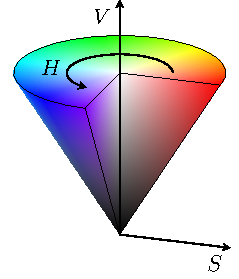
\includegraphics{tikz/hsv_cone/hsv_cone.pdf}
%	\caption{Ο χρωματικός χώρος \en{HSV}.}
%\end{figure}
